\section{Implementation}\label{Sec:Implementation}
In this section we will describe how our data has been setup and how the various methods have been implemented. \autoref{Subsec:TET_features} and \autoref{Subsec:TET_historgram_and_distance} will focus on describing our TET features and how we compare them.
\autoref{Subsec:Metric_Tree_rep} will describe how we use Metric Trees in order to compare a large amount of TETs. We end this section by describing how we implemented node2vec and a brute force comparison method in subsection \autoref{Subsec:n2v_implementation} and \autoref{Subsec:brute_force}.

\subsection{TET Features}
% Indledning:


For each $u$ in the set of all users $U$, we build a TET $T_u$. The root of TET $T_u$ is its corresponding user $u$.
A node $n$ is a user-node in the graph $G$ if $User(n) = True$.

The feature User is in the boolean domain meaning that this feature will be either true or false (\autoref{Eq:Userdomain}).
\begin{equation}\label{Eq:Userdomain}
  User(n)\rightarrow \{True, False\}
\end{equation}


Rating is a feature which is either low, medium or high and the original rating has been split into these three categories.
The original ratings are numerical values between 0 and 5, which was then translated into the new form where $low<2.5\leq mid \leq 3.5<high$.
For each rating, we thus have that:
\begin{equation}\label{Eq:Ratingdomain}
    Rating(u, m) \rightarrow \{Low, Mid, High\}
\end{equation}
Note that \autoref{Eq:Ratingdomain} is the case for every rating in $G$.
Each genre in the dataset is a feature in the boolean domain. These features will return a value when given a movie $m$, returning true if $m$ is categorized as the genre, and false otherwise (\autoref{Eq:genredomain}).
\begin{equation}\label{Eq:genredomain}
\begin{aligned}
Action(m)& \rightarrow \{True, False\} \\
Comedy(m)& \rightarrow \{True, False\} \\
&\vdots \\
Western(m)& \rightarrow \{True, False\} \\
\end{aligned}
\end{equation}

The TETs constructed from the MovieLens dataset will be represented with the structure shown in \autoref{Eq:TETstructure}.
\begin{equation}\label{Eq:TETstructure}
User(u) \stackrel{m}{\longrightarrow} Rating(u,m) \longrightarrow Genre(m)
\end{equation}

The TET will represent a neighborhood of the graph with a User as the root.

The sub-trees are themselves TETs as shown in \autoref{Eq:subtetstructure}.
\begin{equation}\label{Eq:subtetstructure}
\begin{aligned}
Rating(u,m)& \longrightarrow Action(m) \\
Rating(u,m)& \longrightarrow Comedy(m)\\
& \vdots \\
Rating(u,m)& \longrightarrow Western(m)
\end{aligned}
\end{equation}

Since the count of occurrences of \textit{False} values is often semantically not very meaningful, as stated in \cite{jaeger2019counts}, and also are of little relevance in our case, we only consider \textit{True} values. The tree will therefore end up having the form seen in \autoref{fig:Tet_example}

\begin{figure}[H]
    \centering
    \begin{adjustbox}{width=0.5\textwidth}
    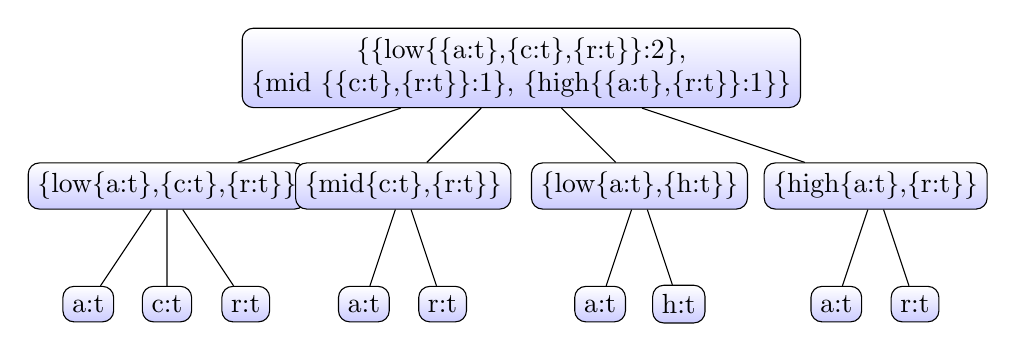
\begin{tikzpicture}[
  	every node/.style = {shape=rectangle, rounded corners,
    draw, align=center,
    top color=white, bottom color=blue!20},
    level 1/.style={sibling distance=3cm},
	level 2/.style={sibling distance=1cm}, 
    ]
  
  \node {\{\{low\{\{a:t\},\{c:t\},\{r:t\}\}:2\},\\
   \{mid \{\{c:t\},\{r:t\}\}:1\}, \{high\{\{a:t\},\{r:t\}\}:1\}\}}
	child{ node{\{low\{a:t\},\{c:t\},\{r:t\}\}} 
		child{ node{a:t}}
		child{ node{c:t}}
		child{ node{r:t}}
		}
	child{ node{\{mid\{c:t\},\{r:t\}\}} 
		child{ node{a:t}}
		child{ node{r:t}}
		}
	child{ node{\{low\{a:t\},\{h:t\}\}} 
		child{ node{a:t}}
		child{ node{h:t}}
		}
    child{ node{\{high\{a:t\},\{r:t\}\}}
	    child { node{a:t}}
      	child { node{r:t}} 
      	}
      ;
\end{tikzpicture}

%
%
%
    \end{adjustbox}
    \caption{TET Tree example}
    \label{fig:Tet_example}
\end{figure}

%The value of a TET T(X) for a user U will be denoted as V(T(U)). If the node U is not a user or is not part of domain, the value for the tree default to false.\todo{this part has to be more precise and telling look at bottom of p.39 in tet article}

The tree can also be represented as \autoref{Eq:TETvector}

\begin{equation}\label{Eq:TETvector}
    T_u=
    \begin{cases}
      (low \{(action:t),(casual:t), (romance:t)\}):2 \\
      (mid \{(comedy:t),(romance:t)\}):1 \\
      (high\{(adventure:t),(romance:t)\}):1
    \end{cases}
\end{equation}

% Where is the action and horror movie?
This tells that the tree $T_u$ has 2 movies with low rating and the genres action, casual, and romance. There is a movie rated in the mid range with genres comedy and romance, and a movie that is highly rated with genres adventure and romance.

With this structure we have a representation of user preferences.
The structures can be compared to find similarities and thereby make more trustworthy recommendations for a user.

\subsection{TET Histograms and Distance}
	Comparing the TET can be done in different ways. One of the method used to find similarity between the TETs is to transform the TET into a histogram is representing the by using the vector representation from \autoref{Eq:TETvector} we can calculate each substructures percentile distribution. this would give a representation as \autoref{fig:Tethistogram}
	
	\begin{figure}[H]
		\centering
		\begin{adjustbox}{width=0.5\textwidth}
			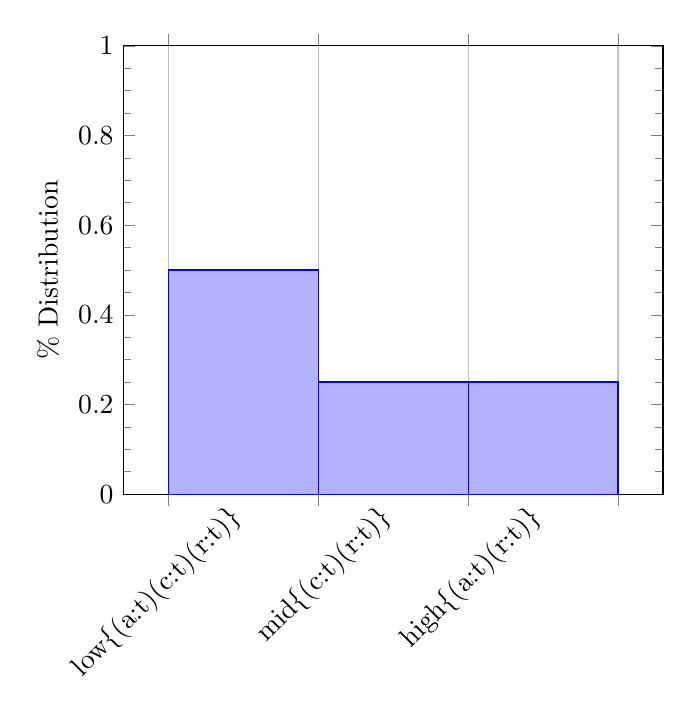
\begin{tikzpicture}
	\begin{axis}[
	ybar interval, 
	ymax=1,ymin=0, 
	minor y tick num = 3,
	ylabel = {\% Distribution},
	symbolic x coords={low\{(a:t)(c:t)(r:t)\}, mid\{(c:t)(r:t)\}, high\{(a:t)(r:t)\}, high\{(y:t)(r:t)\}},
	x tick label style={font=\normalsize, rotate=45, anchor=east},
	]
	\addplot coordinates {(low\{(a:t)(c:t)(r:t)\}, 0.5) (mid\{(c:t)(r:t)\}, 0.25) (high\{(a:t)(r:t)\}, 0.25) (high\{(y:t)(r:t)\}, 0.10)};
	\end{axis}
\end{tikzpicture}

%\begin{tikzpicture}

%\definecolor{bblue}{HTML}{4F81BD}

%\begin{axis}[
%major x tick style = transparent,
%ymin=0,
%bar width=1cm,
%minor y tick num = 3,
%ymajorgrids = true,
%ylabel = {\% distribution},
%symbolic x coords={low\{(a:t)(c:t)(r:t)\}, mid\{(c:t)(r:t)\}, high\{(a:t)(r:t)\}},
%xtick = data,
%x tick label style={font=\normalsize, rotate=45, anchor=east},
%]
%\addplot[ybar , style={bblue,fill=bblue,mark=none}]
%coordinates {(low\{(a:t)(c:t)(r:t)\}, 0.5) (mid\{(c:t)(r:t)\}, 0.25) (high\{(a:t)(r:t)\}, 0.25)};

%\end{axis}
%\end{tikzpicture}
		\end{adjustbox}
		\caption{caption}
		\label{fig:Tethistogram}
	\end{figure}
	
	By using this representation as a vector we can compare two histograms with simple distance measures as forekamle manhatten or euclidean distance.
	
	When comparing two histograms they will most likely have some elements the other does not have the histogram without the element will simply get 0 for the missing value and thereby be able to add distance for the missing element. A simple example done with manhattan distance can be seen in \autoref{Eq:manhattencomparason}.
	
	\begin{equation}\label{Eq:manhattencomparason}
	D(\begin{bmatrix}
	x_{1.1} \\
	x_{1.2} \\
	\end{bmatrix},
	\begin{bmatrix}
	x_{2.1} \\
	x_{2.2} \\
	x_{2.3}
	\end{bmatrix})= |x_{1.1} - x_{2.1}| + |x_{1.2} - x_{2.2}| + |0 - x_{2.1}|
	\end{equation}
	
	This is easily implemented if the vectors are programmed as dictionaries by going through, the union of keywords in the two dictionaries and returning 0 it a key is not found.

\subsection{Metric Tree representation}
  Since we can assume, with good reason, that datasets used in recommender systems only will increase in size, we are interested in minimizing the computation time of structural data queries, like the k-nearest neighbor query.
  In order to find the exact k-nearest neighbors for only one user, we would have to compare the user with all the other users.
  This will result in a linear runtime, which is usually categorized as efficient in the theory of algorithm design and implementation. But since the datasets used in recommender systems tend to be very large, including millions of users, having to calculate the distance between one user and millions of other users may become quite time consuming.
  Furthermore, if each user has to be compared to any other user, a brute force k-nearest neighbor approach will lead to a quadratic runtime.
  As a solution to this problem, we can use the Metric Tree (MT) datastructure for improving nearest neighbor retrieval.
  We refer to \cite{jaeger2019counts} and \cite{uhlmann1991} for the complete definition of MTs, but we give a short explanation of the parts relevant to this paper.

  The Metric Tree is a datastructure that consists of two types of nodes, internal nodes and leaf nodes. An internal node contains two entities and two branches. A leaf node contains a set of entities, also known as the bucket.
  A MT is constructed by a recursive procedure in which a dataset is split. The procedure splits data and recursively calls itself over each of the subsets, until a stopping condition is met.
  If the maximal tree depth is reached, or the current set to be splitted is not larger than the maximal bucket size, a leaf node is returned.
  If not, two entities $z1$ and $z2$ are chosen randomly from the dataset, and data are split by their distances to these entities.

  With the Metric trees implemented, we can use a greedy algorithm for finding the approximate k-nearest-neighbors for a user.
  As stated in \cite{jaeger2019counts}, given a metric tree, the fastest solution for approximate k-nearest-neighbor retrieval for a query object is to traverse the tree, following at each node the branch whose corresponding entity is closer to the query one, until a leaf node is found.
  We can then sort the entities in the bucket contained in the leaf node according to their distance to the query object, and return the k nearest neighbors. We note here that this only is an approximate solution, but it will provide us with results that are more than accurate for recommendation tasks.

\input{Article/Implementation/Node2vec_imp}
\subsection{Brute force comparison}\label{Subsec:brute_force}
One of the most simple methods of comparing users in data set is to compare all relations one by one. 
In an unweighted graph if there was a relation from a user $A$ to a product $p$ and a relation from user $B$ to $p$ there would be a distance $d$ of 0 between these users assuming that this is the only relation user A and B has. 
A weighted graph the distance would also depend on the relation weight, if $A$ has a relation to $p$ with a weight of 2 and $B$ with a relation to $p$ with a weight of 3, using Manhattan distance there would a distance of 1 between $A$ and $B$. 
This can then be extended to all product relations $P$ as seen in \autoref{eq:manhat}

\begin{equation}\label{eq:manhat}
	d(A,B) = \sum_{i=1}^{P} |A_i - B_i|
\end{equation}

